\section{Confidence Intervals for \(\sigma^2\)}

\nl We have $S = \dfrac{1}{n-1} \displaystyle \sum (X_i-\Xbar)^2$ is unbiased and $V = \dfrac{(n-1)S^2}{\sigma^2}$ is a pivotal quantity with $\chi^2$ distribution and $(n-1)$ df.

\nl For a confidence interval, we use
$$\P{\,\chi^2_L \,\leq\, \frac{(n-1)S^2}{\sigma^2} \,\leq \, \chi^2_U \,} = 1 - \alpha$$

\nl As with t-distributions, we need both our $\alpha$ and df $n-1$. But $\chi^2$ itself is not symmetric. \red{The most common C.I. makes symmetric probability in the \say{tails}}
\notab{\begin{center}
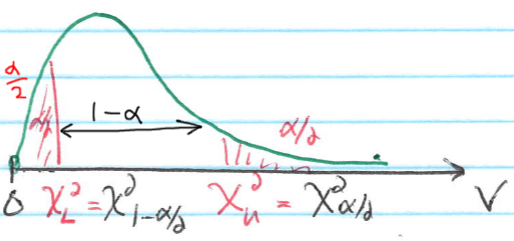
\includegraphics[width=3.5in]{89pic1.png}
\end{center}}
\noindent Then
\begin{align*}
	& \dfrac{\chi^2_L}{(n-1)S^2} \,\leq\, \dfrac{1}{\sigma^2} \,\leq\, \dfrac{\chi^2_U}{(n-1)S^2}\\\\
	\implies & \dfrac{1}{\chi^2_L} \,\geq\, \dfrac{\sigma^2}{(n-1)S^2} \,\geq\, \dfrac{1}{\chi^2_U}\\\\
	\implies & \dfrac{(n-1)S^2}{\chi^2_L} \,\geq\, \sigma^2 \,\geq\, \dfrac{(n-1)S^2}{\chi^2_U}\\\\
	\iff &  \color{red}\boxed{\color{black}  \dfrac{(n-1)S^2}{\chi^2_U} \,\leq\, \sigma^2 \,\leq\, \dfrac{(n-1)S^2}{\chi^2_L}}
\end{align*}
\begin{center}\red{Confidence interval for $\sigma^2$}\end{center}


\newpage
\addcontentsline{toc}{subsection}{Table 6: $\chi^2$ Lower Tail}
\notab{\begin{center} 
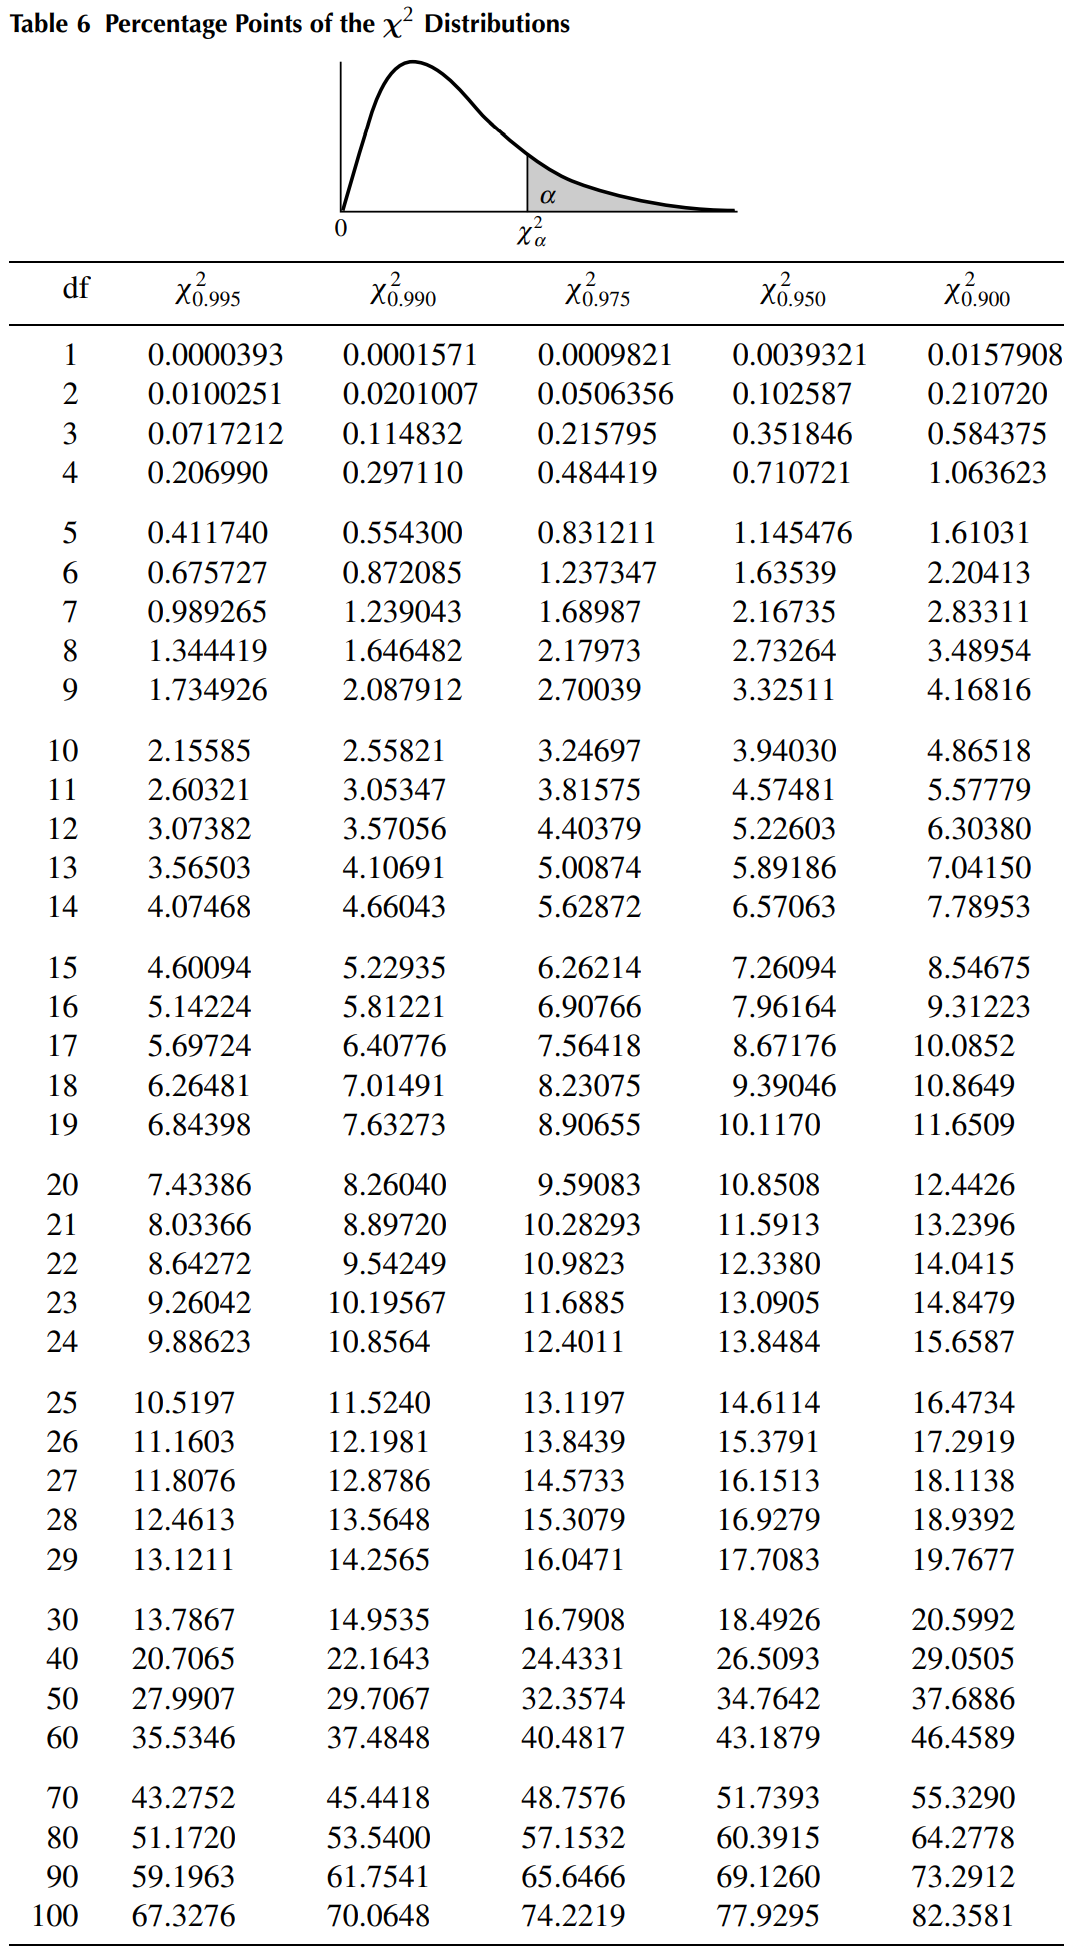
\includegraphics[width=5in]{Table6a.png}
\end{center}}

\newpage
\addcontentsline{toc}{subsection}{Table 6: $\chi^2$ Upper Tail}
\notab{\begin{center}
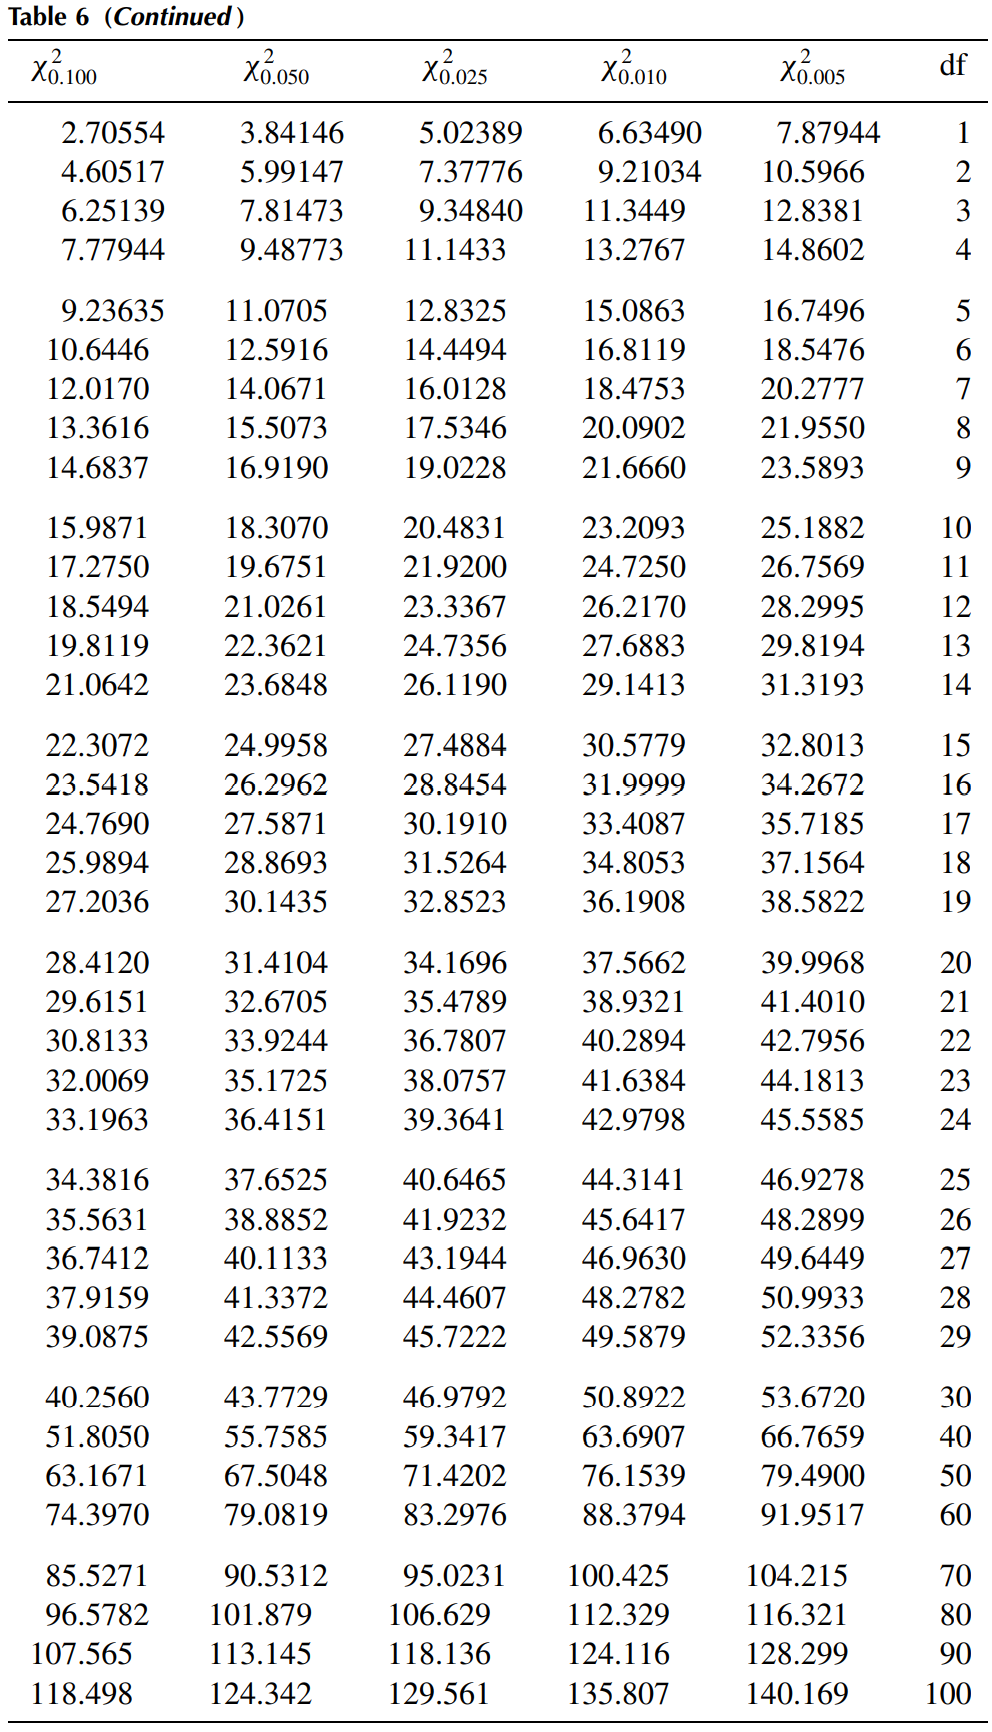
\includegraphics[width=5in]{Table6b.png}
\end{center}}

\newpage

\example Construct a 90\% C.I. for $\mu$ and $\sigma^2$.
$$\underbrace{85.4 \qquad 86.8 \qquad 86.1 \qquad 85.3 \qquad 84.8 \qquad 86.0}_{\textstyle \text{Data set, } n = 6}$$
$$\Xbar = 85.7\overline{3} \qquad S^2 = 0.502\overline{6} \qquad S \approx 0.7089$$
90\% C.I. $\implies \alpha = 0.10, \; \dfrac{\alpha}{2} = 0.05$ with df $n-1 = 5$.
$$\color{blue} \chi^2_L = \chi^2_{0.950} = 1.145476 \qquad \color{ggreen}\chi^2_U = \chi^2_{0.050} = 11.0705\color{black}$$

\nl A common mistake people make is forgetting that the lower bound is $\chi^2_U$. For $\sigma^2$,
\begin{center}
	$\dfrac{5\cdot(0.502\overline{6})}{\color{ggreen}11.0705}\color{black} \, \leq \, \sigma^2 \,\leq\, \dfrac{5\cdot(0.502\overline{6})}{\color{blue}1.145475\color{black}} $

	\nl $0.227 \,\leq\, \sigma^2 \,\leq\, 2.194$
	
	\nl $\sigma^2 \in (0.227,\;2.194)$\end{center}


\nl For $\mu$, use a $t$-distribution with 5 degrees of freedom.
$$\red{\Xbar} \pmp \color{ggreen}t_{0.050}\color{black} \cdot \color{blue}S\color{black}\quad\implies\quad \red{85.7\overline{3}} \pmp (\color{ggreen}2.015\color{black})(\color{blue}0.7089\color{black})$$
$$\mu \in (84.305,\; 87.162)$$